\documentclass[12pt]{article}

\usepackage[brazilian]{babel}
\usepackage[utf8]{inputenc}
\usepackage{graphicx}
\usepackage{mathtools}
\usepackage{amsthm}
\usepackage{thmtools,thm-restate}
\usepackage{amsfonts}
\usepackage{hyperref}
\usepackage[singlelinecheck=false]{caption}
\usepackage[backend=biber,url=true,doi=true,eprint=false,style=numeric]{biblatex}
\usepackage{enumitem}
\usepackage[justification=centering]{caption}
\usepackage{indentfirst}
\usepackage{algorithm}
\usepackage{algpseudocode}
\usepackage{listings}
\usepackage[x11names,rgb,table]{xcolor}
\usepackage{tikz}
\usepackage{hyperref}
\usepackage{subcaption}
\usepackage{booktabs}
\usepackage{linegoal}
\usepackage{geometry}
\usetikzlibrary{snakes,arrows,shapes}

\addbibresource{references.bib}
\graphicspath{{imgs/}}

\makeatletter
\def\subsection{\@startsection{subsection}{3}%
  \z@{.5\linespacing\@plus.7\linespacing}{.1\linespacing}%
  {\normalfont}}
\makeatother

\makeatletter
\patchcmd{\@setauthors}{\MakeUppercase}{}{}{}
\makeatother

\DeclareMathOperator*{\argmin}{arg\,min}
\DeclareMathOperator*{\argmax}{arg\,max}
\DeclareMathOperator*{\Val}{\text{Val}}
\DeclareMathOperator*{\Ch}{\text{Ch}}
\DeclareMathOperator*{\Pa}{\text{Pa}}
\DeclareMathOperator*{\Sc}{\text{Sc}}
\newcommand{\ov}{\overline}
\newcommand{\tsup}{\textsuperscript}

\newcommand\defeq{\mathrel{\overset{\makebox[0pt]{\mbox{\normalfont\tiny\sffamily def}}}{=}}}

\newcommand{\algorithmautorefname}{Algorithm}
\algrenewcommand\algorithmicrequire{\textbf{Input}}
\algrenewcommand\algorithmicensure{\textbf{Output}}
\algnewcommand{\LineComment}[1]{\State\,\(\triangleright\) #1}

\captionsetup[table]{labelsep=space}

\theoremstyle{plain}

\newcounter{dummy-def}\numberwithin{dummy-def}{section}
\newtheorem{definition}[dummy-def]{Definition}
\newcounter{dummy-thm}\numberwithin{dummy-thm}{section}
\newtheorem{theorem}[dummy-thm]{Theorem}
\newcounter{dummy-prop}\numberwithin{dummy-prop}{section}
\newtheorem{proposition}[dummy-prop]{Proposition}
\newcounter{dummy-corollary}\numberwithin{dummy-corollary}{section}
\newtheorem{corollary}[dummy-corollary]{Corollary}
\newcounter{dummy-lemma}\numberwithin{dummy-lemma}{section}
\newtheorem{lemma}[dummy-lemma]{Lemma}
\newcounter{dummy-ex}\numberwithin{dummy-ex}{section}
\newtheorem{exercise}[dummy-ex]{Exercise}
\newcounter{dummy-eg}\numberwithin{dummy-eg}{section}
\newtheorem{example}[dummy-eg]{Example}

\numberwithin{equation}{section}

\newcommand{\set}[1]{\mathbf{#1}}
\newcommand{\pr}{\mathbb{P}}
\newcommand{\eps}{\varepsilon}
\renewcommand{\implies}{\Rightarrow}

\newcommand{\bigo}{\mathcal{O}}

\setlength{\parskip}{1em}

\lstset{frameround=fttt,
	numbers=left,
	breaklines=true,
	keywordstyle=\bfseries,
	basicstyle=\ttfamily,
}

\newcommand{\code}[1]{\lstinline[mathescape=true]{#1}}
\newcommand{\mcode}[1]{\lstinline[mathescape]!#1!}


\title{%
  \vspace{-2.5cm}
  {
\includegraphics[scale=0.2]{logo-usp.png}}\\
  {\textbf{\uppercase{\Large USP --- Universidade de São Paulo}}}\\
  \vspace{2cm}
  {Aprendizagem automática de redes soma-produto}\\
  \vspace{2.5cm}
\flushleft{Candidato: Renato Lui Geh\\
Orientador: Prof.\ Dr.\ Denis Deratani Mauá}\\
  \vspace{2.5cm}
  \centering
  {\textbf{São Paulo}}\\
  \vspace{0.25cm}
  {\textbf{2017}}\\
}
\date{}

\begin{document}

\maketitle

\newgeometry{margin=1in}
\section{Introdução}

Aprendizado de máquina é uma área da Inteligência Artificial cujo objetivo é estatisticamente
ajustar os parâmetros de um certo modelo matemático dado um conjunto de dados a fim de que seja
possível fazer previsões acuradas do que se está modelando. Para isso, faz-se uso de modelos
estatísticos e métodos computacionais. Modelos probabilísticos baseados em grafos (PGM, do inglês
\textit{Probabilistic Graphical Model}), são uma classe destes modelos estatísticos em que se usa
grafos para representá-los graficamente.

Modelos probabilísticos baseados em grafos representam uma distribuição de probabilidade de
forma compacta. Estes modelos representados por grafos facilitam tanto a compreensão humana ao
estudá-los, quanto possibilitam que vários problemas já existentes em Teoria dos Grafos sejam
utilizados como solução para problemas em PGMs. Extrair conhecimento de PGMs é análogo a extrair a
probabilidade de um certo evento ocorrer dado que eventos distintos tenham ocorrido. Tal extração
de conhecimento é chamada de inferência. Fazer inferência exata em PGMs clássicas, ou seja,
acharmos a probabilidade exata de um certo evento, é intratável. Uma solução para este problema é
utilizarmos métodos para inferência aproximada nestes modelos. No entanto, tais algoritmos
aproximados são muitas vezes difíceis de analisar. Além disso, como os algoritmos de aprendizado do
modelo utilizam inferência como subrotina, por consequência o aprendizado torna-se aproximado.

\begin{figure}[h]
  \centering
  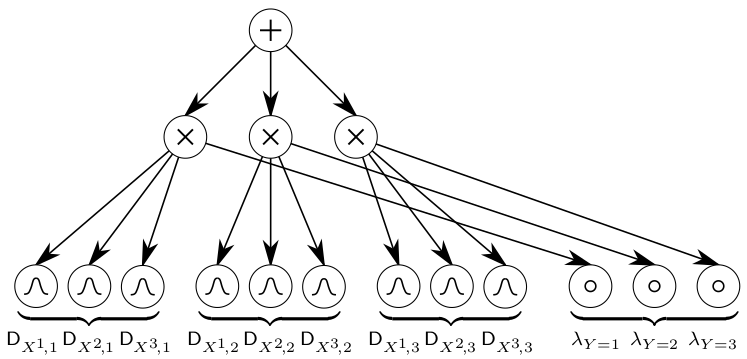
\includegraphics[scale=0.4]{nbayes.png}
  \caption{}\label{spn-example}
\end{figure}

Redes soma-produto (SPN, de \textit{Sum-Product Network}) são PGMs que representam uma distribuição
de probabilidade tratável. Proposto em 2011, SPNs computam inferência exata em tempo linear ao
número de arestas de seu grafo se sua estrutura obedecer a certas propriedades
\cite{poon-domingos}. A~\autoref{spn-example} mostra um exemplo de rede soma-produto representando
o modelo Naïve Bayes com três atributos. SPNs apresentam uma série de características
interessantes, como sua arquitetura profunda que permite representar funções de forma mais
eficiente quanto mais profundo seu grafo~\cite{shallow-vs-deep}. Outras interessantes propriedades
teóricas incluem uma generalização de SPNs para qualquer semianel em que o produto tenha escopo
disjunto~\cite{sp-theorem}. Com relação a aplicações, SPNs tiveram resultados impressionantes em
diversas áreas, como enovelamento de proteínas~\cite{rec-dec-non-convex}, modelagem de
sinais~\cite{model-speech}, classificação e reconstrução de imagens
\cite{gens-domingos,poon-domingos,clustering}, reconhecimento de atividade~\cite{activity} e
linguagem natural~\cite{nat-lang}.

Neste projeto, pretende-se desenvolver uma biblioteca livre e gratuita para inferência e algoritmos
de aprendizado estado-da-arte em SPNs, analisando-se experimentalmente tais algoritmos em tarefas
reais, como compleição e classificação de imagens.

\section{Objetivos}

Os objetivos esperados neste trabalho são:

\begin{enumerate}
  \item Domínio de conceitos sobre aprendizagem de SPNs.
  \item Desenvolvimento de uma biblioteca livre e gratuita de algoritmos de aprendizado de SPNs
    estado-da-arte.
  \item Análise experimental comparativa em tarefas reais.
\end{enumerate}

\section{Metodologia}

A pesquisa terá seu início com o estudo dos conceitos e do estado-da-arte de SPNs. Uma rede
soma-produto pode ser definida como um digrafo acíclico cujos nós podem ser somas ponderadas,
produtos, uma distribuição univariável ou variável indicadora. O escopo de um nó de uma SPN é o
conjunto de todas variáveis que aparecem em seus descendentes. Adicionalmente, para que uma SPN
compute inferência exata, é suficiente que os filhos dos nós somas tenham mesmo escopo e os filhos
de nós produtos tenham escopos disjuntos.

Aprendizado de parâmetros envolve uma estrutura fixa com parâmetros dos nós soma variáveis a fim de
maximizar a verossimilhança do modelo em relação a um conjunto de dados. Similarmente ao
aprendizado paramétrico, o aprendizado estrutural maximiza a verossimilhança descobrindo-se tanto
os pesos quanto a estrutura. Nesta pesquisa, estudar-se-á diferentes métodos de aprendizagem de
SPNs. Primeiro, será iniciado o estudo e implementação do algoritmo de aprendizagem de parâmetros
de Poon e Domingos~\cite{poon-domingos}, replicando-se a estrutura da rede para compleição de
imagens descrita no artigo. Em seguida, serão estudados os algoritmos de aprendizado estrutural
de Ventura e Dennis~\cite{clustering}, Gens e Domingos~\cite{gens-domingos}, e Vergari e di
Mauro~\cite{vergari-mauro}. Após o entendimento de cada algoritmo de aprendizagem, será iniciada a
implementação do algoritmo.

A implementação dos algoritmos será desenvolvida em uma biblioteca gratuita, em código livre e
repositório aberto, buscando documentar o código e elaborar relatórios. Com o desenvolvimento dos
diferentes algoritmos de aprendizagem, pretende-se elaborar relatórios contendo uma comparação
experimental de todos os algoritmos implementados em conjuntos de dados reais.

Durante a realização do projeto, serão elaborados documentos científicos para possível submissão a
ENIAC 2018 e para o acompanhamento geral do desempenho acadêmico do candidato.

O cronograma para o desenvolvimento desta pesquisa segue abaixo.

\begin{table}[h]
  \centering
  \begin{tabular}{|c|c|c|c|c|c|c|}
    \hline
    Atividade/Mês & 1\tsup{o}--2\tsup{o} & 3\tsup{o}--4\tsup{o} & 5\tsup{o}--6\tsup{o} &
    7\tsup{o}--8\tsup{o} & 9\tsup{o}--10\tsup{o} & 11\tsup{o}--12\tsup{o} \\ \hline
    a & $\times$ & & & & & \\ \hline
    b & $\times$ & & & & & \\ \hline
    c & & $\times$ & & & & \\ \hline
    d & & $\times$ & & & & \\ \hline
    e & & & $\times$ & & & \\ \hline
    f & & & & $\times$ & & \\ \hline
    g & $\times$ & $\times$ & $\times$ & $\times$ & & \\ \hline
    h & & & & & $\times$ & \\ \hline
    i & & & & & $\times$ & $\times$ \\ \hline
    j & & & & & & $\times$ \\ \hline
  \end{tabular}
\end{table}

\begin{enumerate}[label=\alph*.]
  \item Estudo de conceitos de SPN\@.
  \item Estudo e implementação do algoritmo de aprendizado de Poon e Domingos (2011)
    \cite{poon-domingos}.
  \item Estudo e replicação da rede para compleção de imagens descrita em Poon e Domingos (2011).
  \item Estudo e implementação do algoritmo de aprendizado de estrutura de Ventura e Dennis (2012)
    \cite{clustering}.
  \item Estudo e implementação do algoritmo de aprendizado de estrutura de Gens e Domingos (2013)
    \cite{gens-domingos}.
  \item Estudo e implementação do algoritmo de aprendizado de estrutura de Vergari e di Mauro
    (2016)~\cite{vergari-mauro}.
  \item Avaliação de desempenho de algoritmos em problemas de compleição de imagem.
  \item Elaboração de artigo para ENIAC 2018.
  \item Relatório e participação no SIICUSP\@.
  \item Disponibilização da biblioteca e documentação do código.
\end{enumerate}

\printbibliography[]

\end{document}
